\documentclass{beamer}

\usetheme{Antibes}
%\usetheme{split}
% this is a template for slides using beamer package
% adapted from slides written by Ramon Medrado
% first version: Ana Bazzan
\usecolortheme[RGB={120,0,0}]{structure}
\setbeamertemplate{blocks}[rounded][shadow=true]
\usepackage[latin1]{inputenc}
\usepackage{ragged2e}
\usepackage{graphicx}
\usepackage{caption}
\usepackage{booktabs}
\usepackage{subfig}
\usepackage{cite}

\begin{document}
\title{Towards an improved place recognition pipeline using depth and color}

\section{Point Clouds}
\frame{\frametitle{Organized Point Clouds}
	\begin{columns}
		\begin{column}{0.5\textwidth}
			\begin{itemize}
				\justifying
				\item Point clouds that resemble an matrix like structure, where data is split into rows and columns;
				\item Adjacent points (pixels) relationship is known, allowing more efficient nearest neighbor operations and lowering the costs of certain algorithms.			
			\end{itemize}
		\end{column}
		\begin{column}{0.5\textwidth}  %%<--- here
			\begin{center}
				\begin{figure}[ht]
					\centering
					\label{figure:fig1}
					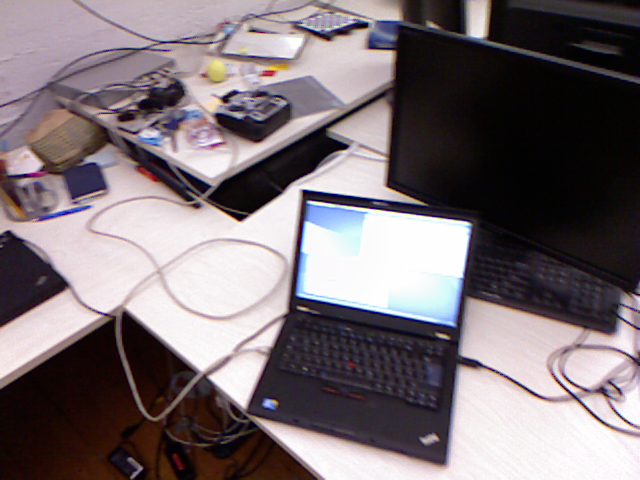
\includegraphics[scale=0.35, height=60pt, width=80pt]{rgb}
					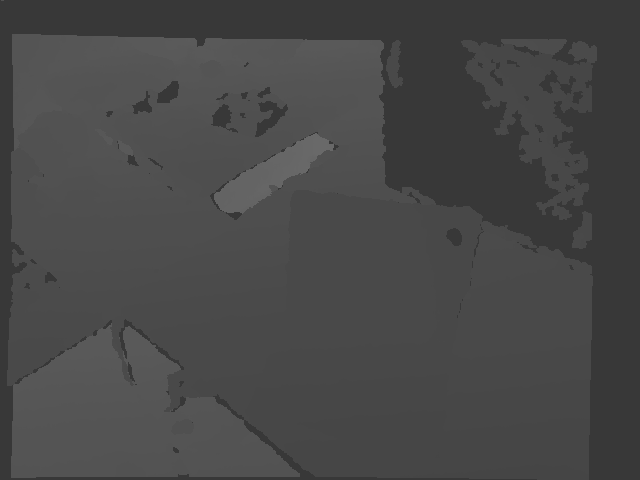
\includegraphics[scale=0.35, height=60pt, width=80pt]{depth}
					
					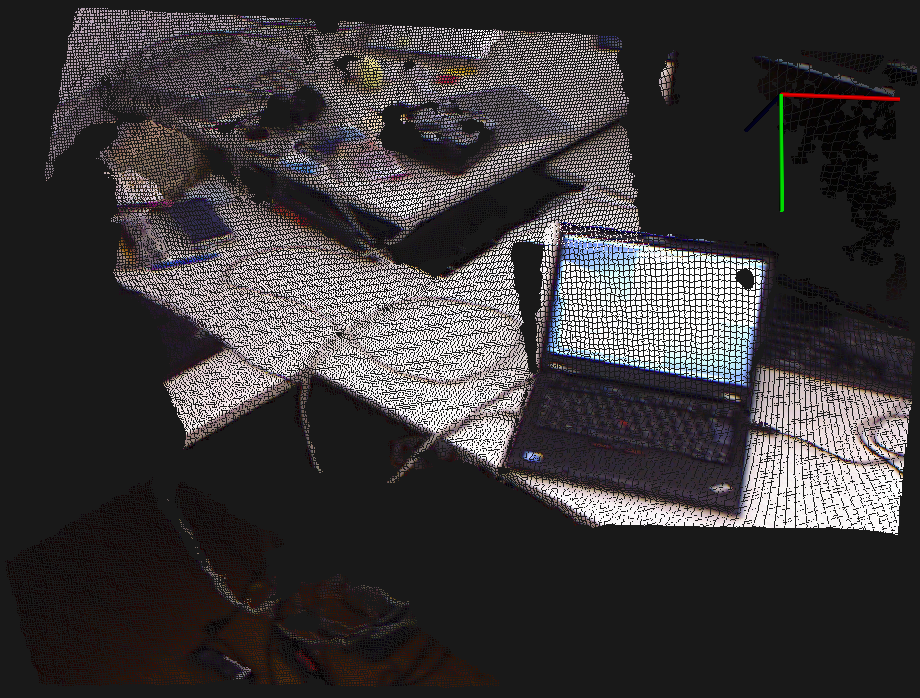
\includegraphics[scale=0.35, height=80pt, width=120pt]{cloud}
					\small
					\caption{RGB, depth and organized point cloud.}	
				\end{figure}
			\end{center}
		\end{column}
	\end{columns}
}
\frame{\frametitle{Unorganized Point Clouds}
	\begin{itemize}
		\justifying
		\item Registration with other point clouds, reconstruction through mesh model conversion etc.
		   
	\end{itemize}	
	
	\begin{figure}[ht]
		\centering
		\label{figure:fig2}
		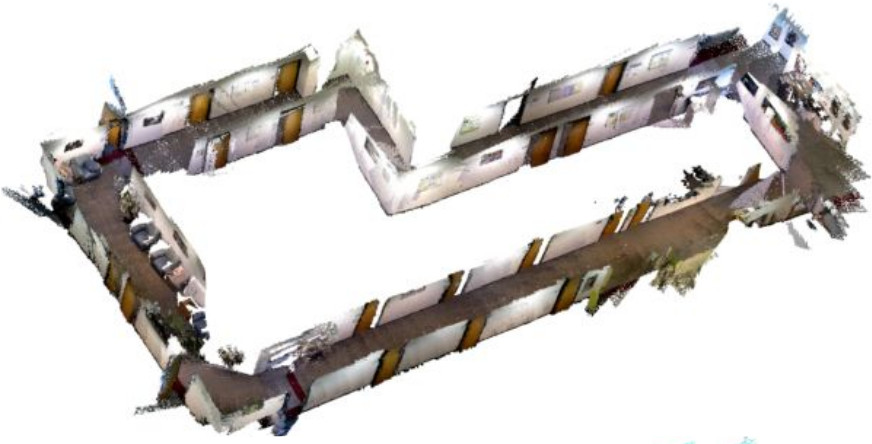
\includegraphics[scale=0.35, height=120pt, width=260pt]{unorganized}		
	\end{figure}
}

\section{How I Ended Up Here}
\frame{\frametitle{How I Ended Up Here}	
	\listoffigures
	\captionsetup{font=normalsize,labelfont={bf,sf}}
	\captionsetup[sub]{font=small,labelfont={bf,sf}}
	
	\begin{itemize}
		\justifying
		\item Reading through some 2013+ SLAM proposals, place recognition or mapping-specific works that make use of depth/point cloud features:
		\begin{itemize}
			\item Keyframe-based Dense Planar SLAM, Ming et al. - ICRA 2017;
			\item CPA-SLAM: Consistent plane-model alignment for direct RGB-D SLAM, Lingnin et al. - ICRA 2016; 
			\item Place recognition based on matching of planar surfaces and line segments, Cupec et al. - IJRR 2015;			
			\item Fast place recognition with plane-based maps, Fern�ndez-Moral et al. - ICRA 2013;
			\item Some object/semantic or keypoint-based works, and skipping through lots of BoW and CNN stuff.   
		\end{itemize}
	\end{itemize}
}

\section{Planar Surface Segmentation Step}
\frame{\frametitle{Current Planar Surface Segmentation Step}	
	\listoffigures
	\captionsetup{font=normalsize,labelfont={bf,sf}}
	\captionsetup[sub]{font=small,labelfont={bf,sf}}
	\begin{itemize}
		\justifying
		\item Fast Plane Extraction in Organized Point Clouds Using Agglomerative Hierarchical Clustering, Feng et al. - ICRA 2014;
		\item Build a graph by dividing a point cloud into several uniform-sized non-overlapped regions:
	\end{itemize}			
			
	\begin{figure}[ht]
		\centering
		\label{figure:fig3}
		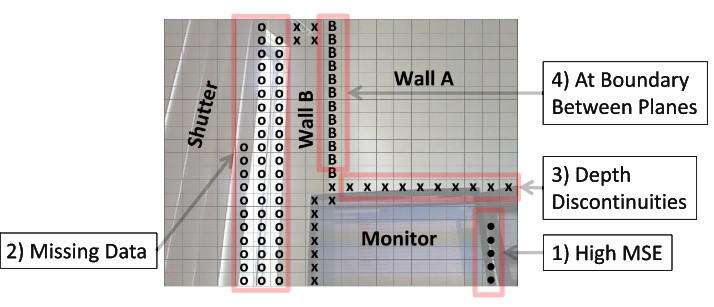
\includegraphics[scale=0.35, height=120pt, width=280pt]{ahc1}		
	\end{figure}			
}
\frame{\frametitle{Current Planar Surface Segmentation Step}	
	\listoffigures
	\captionsetup{font=normalsize,labelfont={bf,sf}}
	\captionsetup[sub]{font=small,labelfont={bf,sf}}
	\begin{itemize}
		\justifying
		\item Find the region with min. plane fitting mean squared error and merge it (edge contraction) with one neighbor such that merge results in the minimum plane fitting MSE:
	\end{itemize}			
	
	\begin{figure}[ht]
		\centering
		\label{figure:fig4}
		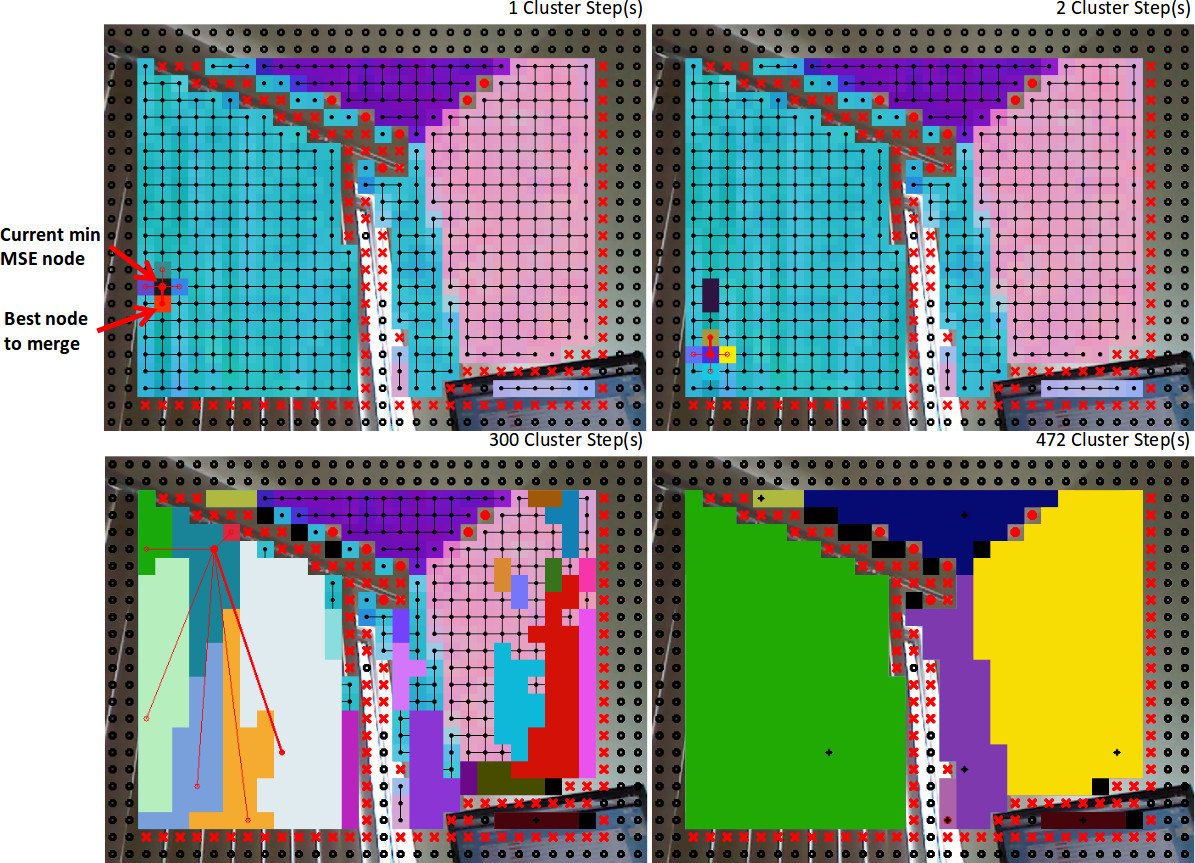
\includegraphics[scale=0.35, height=150pt, width=280pt]{ahc2}		
	\end{figure}			
}
\frame{\frametitle{Current Planar Surface Segmentation Step}	
	\listoffigures
	\captionsetup{font=normalsize,labelfont={bf,sf}}
	\captionsetup[sub]{font=small,labelfont={bf,sf}}
	\begin{itemize}
		\justifying
		\item Refine boundaries of clustered regions with pixel-wise region-growing (only boundary blocks and points):
	\end{itemize}			
	
	\begin{figure}[ht]
		\centering
		\label{figure:fig5}
		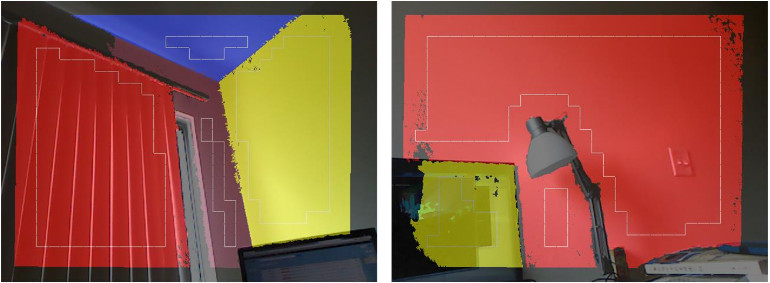
\includegraphics[scale=0.35, height=100pt, width=260pt]{ahc3}		
	\end{figure}			
}	
\frame{\frametitle{Previous Planar Surface Segmentation Step}	
	\listoffigures
	\captionsetup{font=normalsize,labelfont={bf,sf}}
	\captionsetup[sub]{font=small,labelfont={bf,sf}}
	\begin{itemize}
		\justifying
		\item Efficient Organized Point Cloud Segmentation with Connected Components, Trevor et al. - ICRA 2013 Workshop:
		\begin{itemize}
			\item Compute per point normal using Integral Image Normal Estimation (Holzer et al 2012) method;		
			\item Partition into regions with labeled points, attempting to merge with different labeled neighbors;
			\item Detect surfaces with smoothly changing surface normals, within threshold;
			\item Plane fitting using least squares for each region with min. inliers;
			\item Filter regions with exceeding max. threshold curvature.
		\end{itemize}
	\end{itemize}						
}	

\section{Plane Matching}
\frame{\frametitle{Unsure How to Proceed..}	
	\listoffigures
	\captionsetup{font=normalsize,labelfont={bf,sf}}
	\captionsetup[sub]{font=small,labelfont={bf,sf}}
	\begin{itemize}
		\justifying
		\item Fast place recognition with plane-based maps, Fern�ndez-Moral et al. - ICRA 2013;
	\begin{figure}[ht]
		\centering
		\label{figure:fig6}
		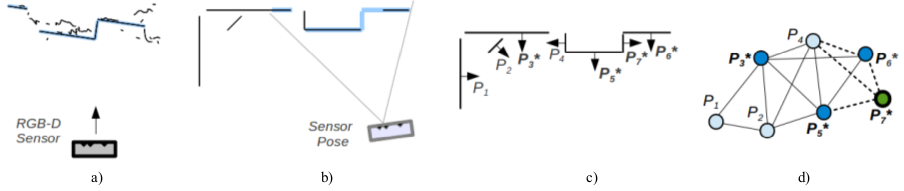
\includegraphics[scale=0.35, height=40pt, width=220pt]{pbmap}		
	\end{figure}
		\item Location Graphs for Visual Place Recognition, Stumm et al. - ICRA 2016;
	\begin{figure}[ht]
		\centering
		\label{figure:fig7}
		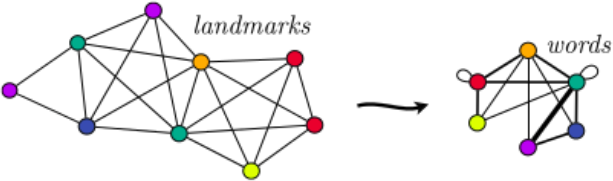
\includegraphics[scale=0.35, height=40pt, width=140pt]{constellationwords}		
	\end{figure}
		\item Searching for more alternatives and/or new ideas.		
	\end{itemize}						
}

\section{Unrelated}
\frame{\frametitle{Unrelated, but important nonetheless}	
	\listoffigures
	\captionsetup{font=normalsize,labelfont={bf,sf}}
	\captionsetup[sub]{font=small,labelfont={bf,sf}}
	\begin{itemize}
		\justifying
		\item Large-Scale 3D Scene Reconstruction with Hilbert Maps, Guizilini and Ramos - IROS 2016:
		\begin{itemize}
			\item HM - Represent input space at an arbitrary resolution while capturing statistical relationships between measurements;
			\item LARD-HM - Localized automatic relevance determination, a new method for the automatic selection of feature coordinate locations (vs OctoMap);
			\item Experiments performed on a 8x2.50GHz notebook with OpenMP parallelization (avg. query time 849ms);
		\end{itemize}
		\item Unsupervised Feature Learning for 3D Scene Reconstruction with Occupancy Maps, Guizilini and Ramos - AAAI 2017:
		\begin{itemize}
			\item PS-HM - Segment planar surfaces based on raw unorganized point cloud data aiming a compact representation of HM (vs LARD-HM, OctoMap).
		\end{itemize}	
	\end{itemize}			
	
			
}

\nocite{*}

\end{document}




